\chapter{MATERIALS AND METHODS - Yeast8}

\section{Consensus \emph{S. cerevisiae} Metabolic Model}
Variety of \emph{S. cerevisiae} genome-scale metabolic models have been used since 2003, and each reconstructed model introduced more manual curations, increasing gene numbers from annotations and better predictions regarding the previous ones \cite{lopes2017genome}. A consensus genome-scale metabolic model of \emph{S. cerevisiae}, Yeast8, is presented in an open-source, version-controlled maintainable way in 2019, claiming that the model can be represented and investigated in a systematic way using Git (https://git-scm.com/) and GitHub (https://github.com/) as a hosting service for the model repository \cite{lu2019consensus}. Systematic way of Yeast8 enables to study simultaneously in collaborative studies, provides record keeping of model changes, version updates, where each version of can be released periodically and accessible all the time (Figure \ref{fig:yeast8_github}).

Yeast8 model can be considered as an updated version of Yeast7 \cite{aung2013revising} with additional corrections based on the annotations available in KEGG and ChEBI, and several gene inclusions from the model iSce926 \cite{chowdhury2015using}. Final version of Yeast8, version 8.3.4 released on July 28, has 3991 reactions, 2691 metabolites, 1149 genes, 14 intracellular compartments.

All simulations in this chapter are done using Yeast8 v8.3.4 model which is hosted in Github (https://github.com/SysBioChalmers/yeast-GEM).

\begin{figure}[H]
\begin{center}
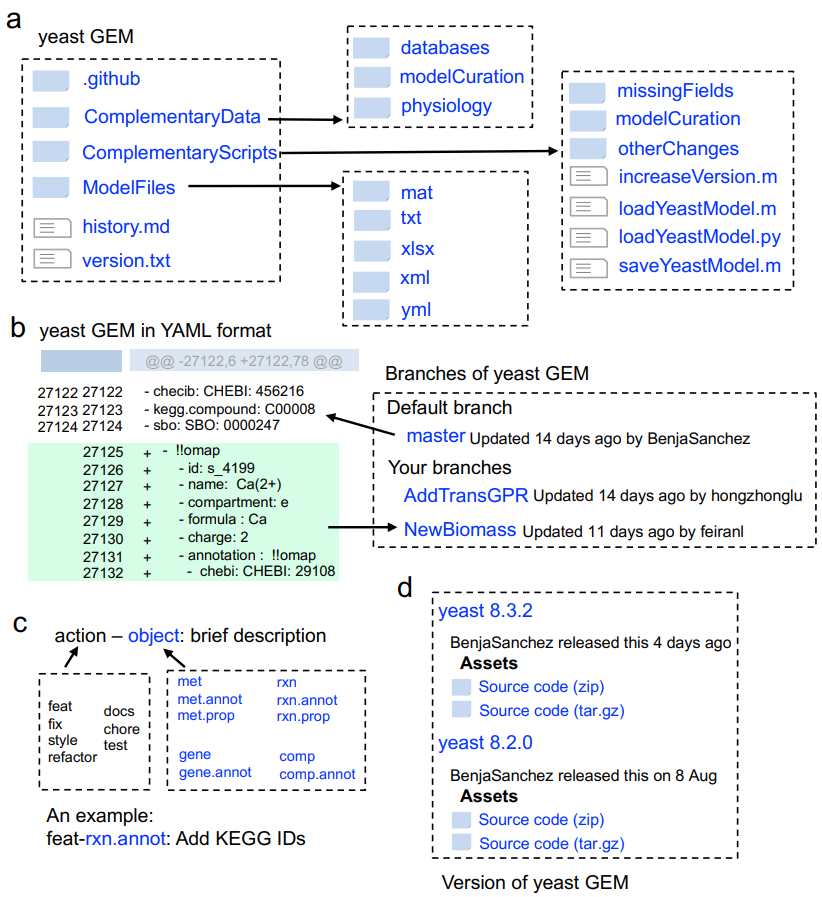
\includegraphics[width=0.9\columnwidth]{yeast8_github.png}
\end{center}
\caption[Repository of yeast GEM on GitHub]{Repository of yeast GEM on GitHub. Figure is taken from \cite{lu2019consensus}. ~ will be redrawned in thesis}
\label{fig:yeast8_github}
\end{figure}

\section{Chemostat Simulation: GAM Fitting}
In order to make sure the \emph{in-silico} obtained growth rate predictions are in agreement with the physiological kinetic parameters obtained from real experiments, fine adjustment on the energy reactions is a requirement. Since the growth-associated maintenance (GAM) and non-growth associated maintenance (NGAM) energy reactions play a determinant role in simulations, fluxes through these reactions must be constrained to a fixed value. Flux of NGAM is constrained to 0.7 mmol gDWh\textsuperscript{-1} for aerobic, and 0 mmol gDWh\textsuperscript{-1} for anaerobic simulations as calculated in the previous studies \cite{nilsson2016metabolic}. For the estimatation of GAM, since it depends on the biomass composition, findings of a chemostat experiment \cite{van1998effect} is used as a guide to fit predictions to. Model is simulated iteratively with a range of values for GAM, and the best fit is found at the level of 55.25 mmol gDWh\textsuperscript{-1} (Figure \ref{fig:Gam_fitting}), GAM flux is constrained accordingly.

\begin{figure}[H]
\begin{center}
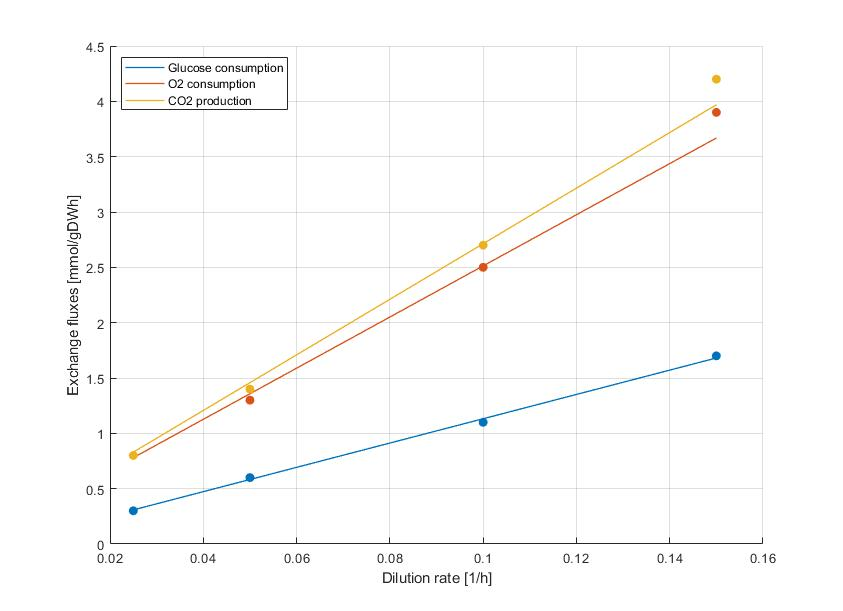
\includegraphics[width=0.8\columnwidth]{Gam_fitting.jpg}
\end{center}
\caption[Chemostat simulation to re-fit growth associated maintenance]{Chemostat simulation to re-fit growth associated maintenance.}
\label{fig:Gam_fitting}
\end{figure}


\section{Flux Balance Analysis}
Flux balance analysis (FBA) assumes that the living cells act as they optimized their lives towards some goal, and as if they were at steady state. To be more clear, steady-state assumption indicates that the metabolites are both produced and consumed at the same rate in a cell, without an accumulation. Therefore, in this system, metabolites are constrained by only the stoichiometric coefficients arised from mass balance of metabolites. As a result of this assumption, FBA solves a set of ordinary differential equations regarding to the stoichiometric matrix:
\begin{equation}
  \ S_{m \times n} \cdot v=0
\end{equation}
\noindent where S is the matrix of the stoichiometric reaction coefficients with m number of metabolites (as rows) and n number of reactions (as columns), and v is the vector of all associated reaction fluxes (mmol/gDWh). Because the matrix S usually has more reactions than metabolites (m<n), the system can result multiple solutions, and being called an underdetermined system. To solve it for an optimal solution, additional constraints are required.

A "growth reaction" is usually included in the reactions of the system to represent the "goal" in the definition of living systems. Growth reactions act as the final consumption of metabolites necessary for the biomass production or cell replication. Additional to the growth, several exchange reactions (uptake or secretion of metabolites from or into extracellular space) are also included. Since the concentrations of extracellular metabolites are measurable experimentall, constraints can be applied to exchange reaction fluxes to shrink solution space. The more constraints introduced into the system, such as reversibility of reactions or known rate values, result smaller solution space. The growth reaction is usually used as an objective function to determine a unique solution from this solution space. The linear problem appears as:
\begin{equation}
  \begin{align}
  \ \text{max}_v \quad & c^T \cdot v \\
  \ \text{subject to} \quad & S_{m \times n} \cdot v=0 \\
  \ & v_{lb} \leq v \leq v_{ub}
  \label{eq:fba}
  \end{align}
\end{equation}
\noindent where c is the objective function vector, v is the vector of fluxes, S is the stoichiometric matrix as above equation. Subscripts lb and ub are the lower and upper boundaries on v. These constraints defines a feasible region of the problem.

In order to simulate batch conditions where minimal yeast medium is used, all the exchange reactions in the model are blocked first (lower bounds are set to 0). Then, only the exchange reactions of ions that are available to the cells in the experimental design (ammonium, phosphate, sulphate, iron(2+), H+, water, chloride, Mn\textsuperscript{2+}, Zn\textsuperscript{2+}, Mg\textsuperscript{2+}, sodium, Cu2\textsuperscript{2+}, Ca\textsuperscript{2+}, potassium) are set free (lower bounds are set to -1000), means that cells can uptake as it needs. While oxygen and glucose uptake rates decreased from 20 mmol gDWh\textsuperscript{-1} and increased to 20 mmol gDWh\textsuperscript{-1}, respectively, fluxes of ethanol, acetate, glycerol, formate, succinate secretion reactions with the growth rate is collected (Figure \ref{fig:fba}).
\hl{I need to show experimental results -preferably from the same article where I got expression data- on the figure to compare with my FBA results}


\begin{figure}[H]
\begin{center}
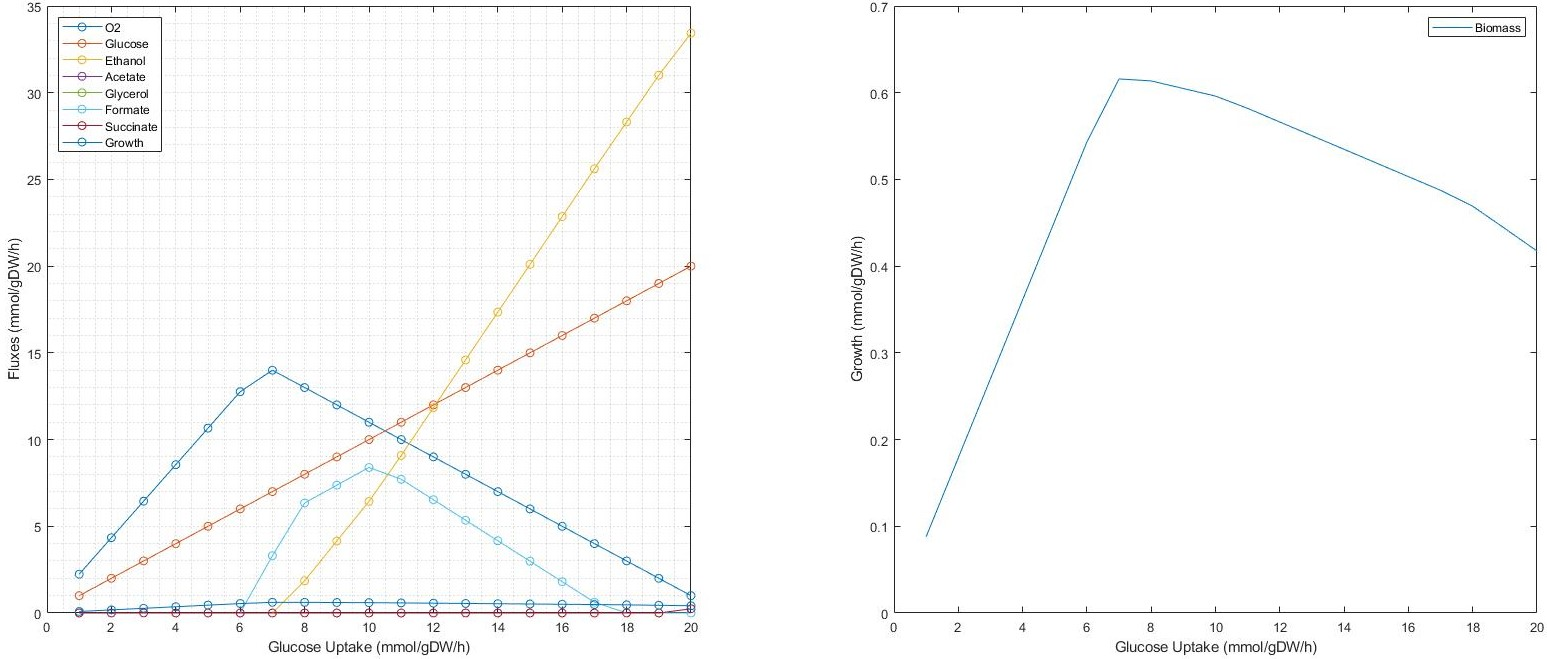
\includegraphics[width=1\columnwidth]{fba.jpg}
\end{center}
\caption[Flux balance simulation results]{Flux balance simulation results where oxygen uptake rate decreased and glucose uptake rate is increased simultaneously. Flux rates of several metabolites on the left, predicted growth rate on the right.}
\label{fig:fba}
\end{figure}


\section{Flux Variability Analysis}
Flux variability analysis (FVA) finds the minimum and maximum available fluxes for each reaction while obeying the provided constraints (for example fixed glucose uptake or growth rate). FVA is mainly used to evaluate the robustness of the model \cite{thiele2010functional}, to find alternative optimum states \cite{mahadevan2003effects}, to check flux distributions when growth is not at optimum level \cite{reed2004genome}, and it has many other applications \cite{gudmundsson2010computationally}.

FVA, similar to FBA, solves two optimization problems for each reaction:
\begin{equation}
  \begin{align}
  \ \text{max}_v / \text{min}_v \quad & v_i \\
  \ \text{subject to} \quad & S_{m \times n} \cdot v=0 \\
  \ & w^T \cdot v \geq  \gamma \cdot Z_0 \\
  \ & v_{lb} \leq v \leq v_{ub}
  \end{align}
\end{equation}
\noindent where $w$ is the objective function equals to $c$ in the problem \ref{eq:fba}, $Z_0 = w^T \cdot v_0$ describes an optimal solution to the problem \ref{eq:fba}, $\gamma$ is an indicator to check whether the FVA is done at the optimal state (where objective flux is the same and $\gamma = 1$) or any other state (where $0 \leq \gamma < 1$).

Flux variabilites of Yeast8 reactions are analyzed by solving the linear problem with the objective functions to minimize and maximize all reactions iteratively with tolerance value of 1e-9 using the GUROBI solver. Minimum and maximum available fluxes are collected in the iterative process for each reaction, and results are plotted for glycolysis, pentose phosphate pathway and TCA pathway reactions as error boxes (Figure \ref{fig:fva}). Flux values obtained through the ordinary FBA solution are also shown as a line.

\begin{figure}[H]
\begin{center}
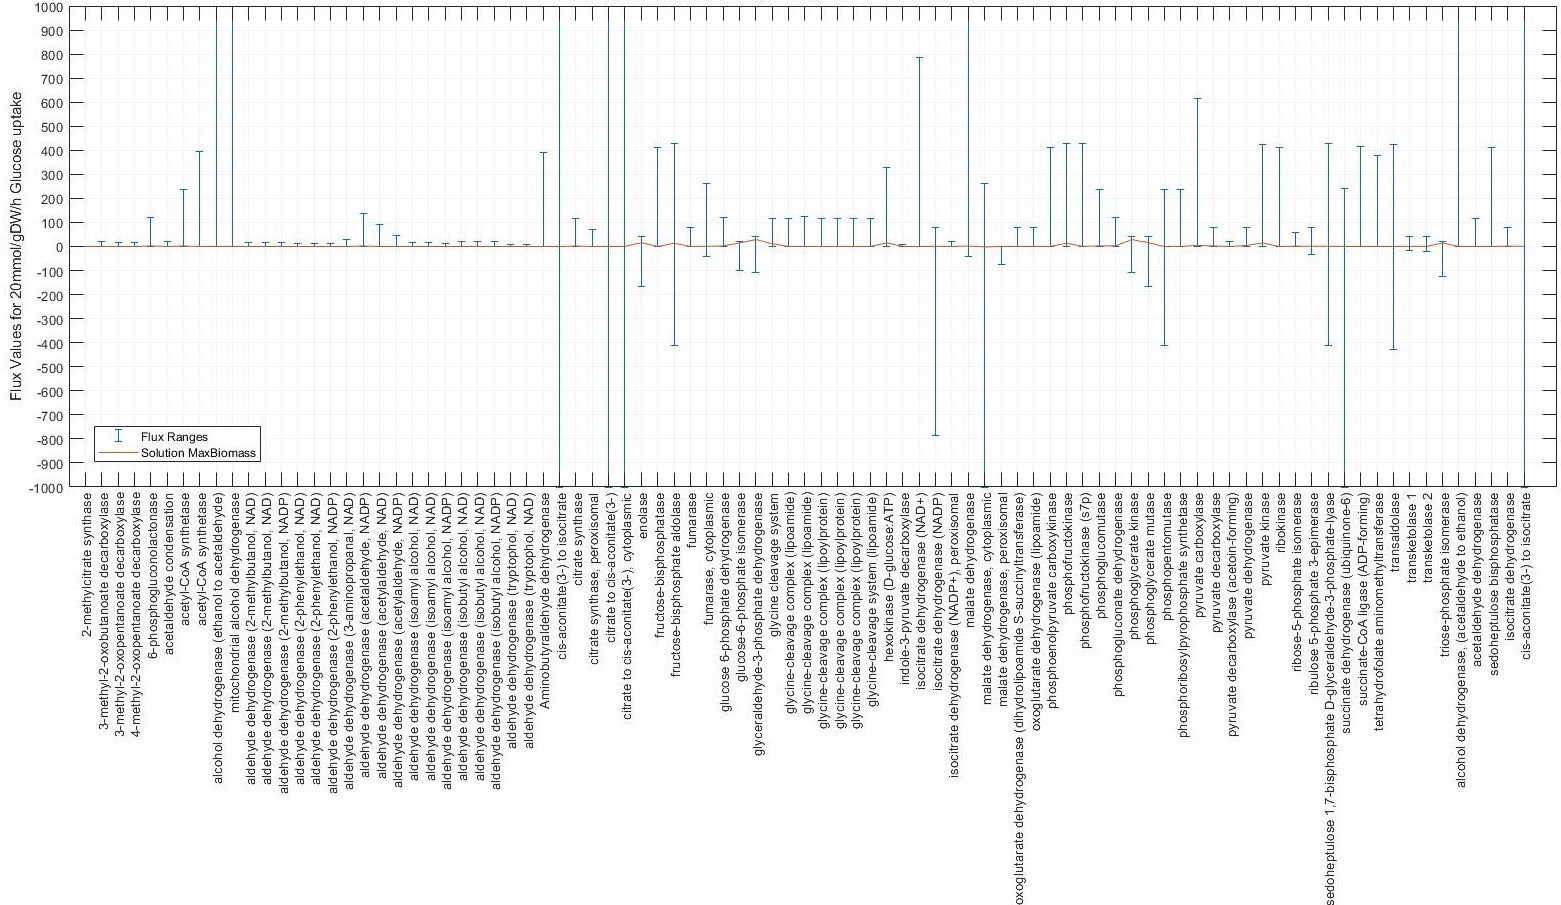
\includegraphics[width=1\columnwidth]{fva.jpg}
\end{center}
\caption[Minimum and maximum fluxes of Glycolysis, PPP and TCA reactions]{Minimum and maximum fluxes of Glycolysis, PPP and TCA reactions.}
\label{fig:fva}
\end{figure}

\section{Phenotype Phase Plane Construction}
\section{ACHRB Sampling}
\section{Expression Data Analysis}
\section{Integration of Expression Data Into Model}
